\chapter{Clusterização} \label{cap:clusterizacao}

A clusterização é denominada como técnica para organização ou agrupamento de uma coleção de padrões, ou elementos que sigam padrões, em \textit{clusters} baseada em similaridade.
Trata-se de uma técnica bastante utilizada em análise exploratórias, agrupamentos, tomada de decisão e implementações de \textit{machine learning}, como:
mineração de dados, recuperação de documentos, segmentação de imagens e padronização \cite{clustering_review}.

\citeonline{tan2013data} definem a análise de \textit{clusters}, ou clusterização, como a ação que agrupa objetos de dados baseado apenas nas informações contidas
nos dados do próprio objeto que permitam descrever os objetos e suas relações. 

Classificação é o processo de encontrar um modelo que possa descrever e distinguir classes de dados \cite{han2011data}.

\citeonline{tan2013data}, \citeonline{han2011data} ressaltam a diferença entre classificação supervisionada e classificação não supervisionada.
Na classificação supervisionada os objetos de dados são analisados a partir de rótulos de classe predefinidos nos objetos, ou seja, 
com as classes de dados previamente definidas e conhecidas. \citeonline{han2011data} chamam este tipo de dado de "dado treinado"
(dados cujos rótulos são conhecidos), onde o modelo que o descreve é obtido a partir da análise dos rótulos.
Na classificação não supervisionada, os rótulos de classe são obtidos a partir da análise dos dados dos objetos, tão somente \cite{tan2013data}.

A clusterização geralmente se refere a este último tipo de classificação \cite{tan2013data}, onde os rótulos de classes dos objetos podem não existir ainda e 
o método empregado na clusterização pode gerar rótulos para um grupo de dados do conjunto \cite{han2011data}.

Os objetos são agrupados (ou "clusterizados") buscando maximizar a similaridade intraclasse e minimizar a similaridade interclasse.
Em outras palavras, o objetivo é formar \textit{clusters} cujos elementos tenham alta similaridade entre si em um mesmo \textit{cluster} 
e baixa similaridade a elementos de outros \textit{clusters} \cite{han2011data}. Por fim, um \textit{cluster} pode ser visto como uma
classe de objetos de onde se é possível derivar regras para o grupo \cite{han2011data}.

Apesar de parecer lógico e simples querer maximizar a similaridade intraclasse e minimizar a similaridade interclasse entre um conjunto de dados, 
\citeonline{tan2013data} exemplificam o quão difícil esta tarefa pode ser na Figura \ref{fig:clusters_difficulty}, onde temos um conjunto
de pontos (a) que pode ser agrupado de formas diferentes gerando quantidades diferentes de \textit{clusters} (b, c, d).

\begin{figure}[h!]
\centering
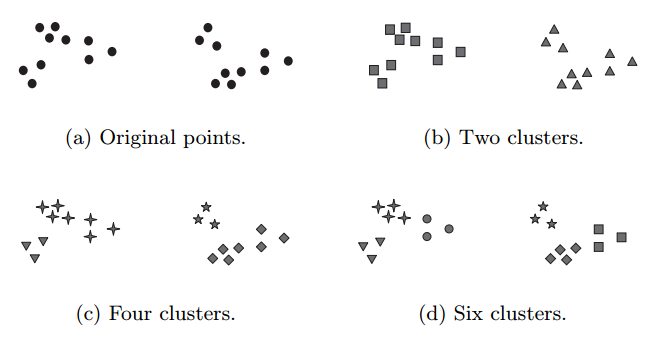
\includegraphics[scale=0.4]{figuras/clusters_difficulty.png}
\caption{Formas de se agrupar o mesmo conjunto de dados. Fonte: \cite{tan2013data}}
\label{fig:clusters_difficulty}
\end{figure}

A aplicação da técnica pode ser resumida nos passos apresentados na Figura \ref{fig:tasks_clustering}.

\begin{figure}[h!]
\centering
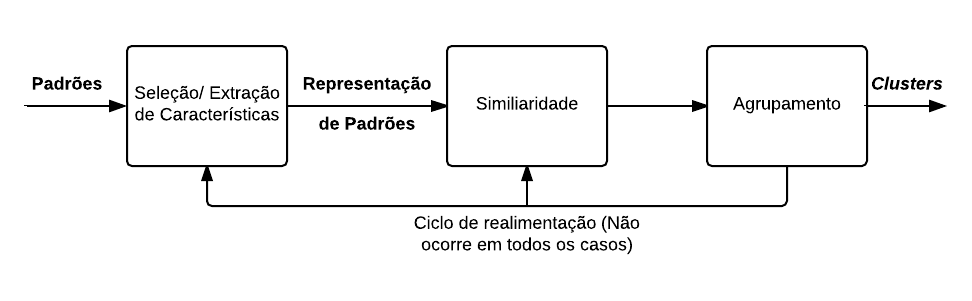
\includegraphics[scale=0.6]{figuras/tasks_clustering.png}
\caption{Passos para clusterização. Adaptado de \citeonline{clustering_review}}
\label{fig:tasks_clustering}
\end{figure}

A representação de padrões está relacionada ao número de classes, número de padrões disponíveis e o número, tipo e escala
das características disponíveis no algoritmo de clusterização. Algumas dessas informações podem não ser controladas pelos
profissionais \cite{clustering_review}.

A seleção de características é o processo de identificação do subconjunto das características mais eficaz para a clusterização, já a extração
de características é o uso de uma ou mais transformações das características de entrada para produzir novas características \cite{clustering_review}.

A similaridade, em geral, é medida por uma função de distância entre um par de padrões ou elementos. Essa função de distância pode variar de acordo com o contexto da aplicação. E por fim, o agrupamento pode ser realizado com uso de inúmeras técnicas e algoritmos diferentes que serão apresentadas nas próximas seções \cite{clustering_review}.

\section{Tipos de clusterização}

A técnica de clusterização pode ser dividida em alguns tipos: hierárquica ou particional; exclusiva, sobreposta ou \textit{fuzzy}; completa ou parcial \cite{tan2013data, clustering_review}. 

\citeonline{clustering_review} definem uma clusterização hierárquica quando ela produz uma série
de partições aninhadas baseadas em um critério para junção ou separação dos \textit{clusters} por meio de similaridade. \citeonline{tan2013data} afirmam que esse tipo de clusterização acontece quando algoritmo
produz um resultado no qual é possível obter \textit{subclusters} e dessa forma os \textit{clusters} são aninhados
e organizados como uma árvore, seguindo a ideia de hierarquia.

Já na clusterização particional o agrupamento dos objetos de dados é realizado em simples \textit{clusters}, os quais pertencem apenas a um \textit{cluster} \cite{tan2013data}.

No processo de clusterização, os objetos de dados podem pertencer a um único \textit{cluster} exclusivamente ou podem
pertencer a diferentes \textit{clusters} ao mesmo tempo. O primeiro caso é conhecido como clusterização exclusiva e o segundo como sobreposta \cite{tan2013data}. Já o tipo \textit{fuzzy} trata da pertinência dos objetos a um grupo de forma probabilística, ou em um grau de pertinência, em vez de determinar se o objeto pertence ou não àquele grupo \cite{tan2013data, clustering_review}.

Por fim, \citeonline{tan2013data} definem uma clusterização como completa quando no resultado todos os objetos estão em pelo menos um grupo. Pois, na clusterização parcial alguns elementos podem ficar sem grupo caso não sejam compatíveis com algum \textit{cluster} formado.

\section{Algoritmos de clusterização}